\def\checkmark{\tikz\fill[scale=0.4](0,.35) -- (.25,0) -- (1,.7) -- (.25,.15) -- cycle;}

\chapter{\ifproject%
      \ifenglish Experimentation and Results\else การทดลองและผลลัพธ์\fi
  \else%
      \ifenglish System Evaluation\else การประเมินระบบ\fi
  \fi}

\section{คำอธิบายการทดลอง}
ในการทดลองนี้เราจะใช้ระบบที่เราสร้างขึ้นมาในการทำการทดสอบโดยใช้เงินตั้งต้น 3,000 USD และทดสอบบนตลาด Crypto Currency (BTC, ETH, BNB) และตลาดหุ้น NASDAQ (AAPL, IBM, JPM, MSFT, NKE, TSLA) ซึ่งเงินตั้งต้นจะถูกแบ่งให้เท่าๆ กันจาก 3,000 USD สำหรับแต่ละเหรียญหรือหุ้นในทั้ง 2 ตลาด โดยวิธีการเข้าซื้อจะมีดังนี้

\begin{table}[ht]
    \centering
    \resizebox{\columnwidth}{!}{%
        \begin{tabular}{lccccc}
            \textbf{ส่วนเสริม}                                                                                                         &
            \multicolumn{1}{l}{\textbf{Classical}}                                                                                   &
            \multicolumn{1}{l}{\textbf{Fuzzy}}                                                                                       &
            \multicolumn{1}{l}{\textbf{Fuzzy C}}                                                                                     &
            \multicolumn{1}{l}{\textbf{Fuzzy PSO}}                                                                                   &
            \multicolumn{1}{l}{\textbf{Fuzzy PSO}}                                                                                                                                           \\
            ใช้ Fuzzy Logic ในการทำอินดิเคเตอร์ขึ้นมา                                                                                       &   & \checkmark &            & \checkmark & \checkmark \\
            \begin{tabular}[c]{@{}l@{}}การจัดการเงินทุนโดยใช้ค่าของอินดิเคเตอร์จาก  Fuzzy Logic\\ (Liquidation F)\end{tabular}               &   &            & \checkmark &            & \checkmark \\
            \begin{tabular}[c]{@{}l@{}}การใช้ Particle Swarm Optimization (PSO) ในการปรับค่าของตัว\\ แปรทางภาษาของอินดิเคเตอร์\end{tabular} &   &            &            & \checkmark & \checkmark
        \end{tabular}%
    }
    \caption{ตัวชี้วัดที่นำมาใช้ในการเข้าซื้อ}
    \label{tab:indicators}
\end{table}
โดยสำหรับวิธี Classical นั้นเราจะใช้ค่าของอินดิเคเตอร์แต่ละตัวตรงๆ มาใช้ตัดสินใจเข้าซื้อ และการใช้ PSO ในการปรับค่าของตัวแปรทางภาษาจะมีพารามิเตอร์ตังนี้
\begin{itemize}
    \item {จำนวนกลุ่ม (Swarm Size) ที่ใช้ในการฝึกสอน จะมี 3 รูปแบบ คือ 5, 10, 15}
    \item {จำนวนสมาชิกในแต่ละกลุ่ม (Number of Particles) จะเป็น 10}
    \item {เงื่อนไขในการจบการทำงาน คือเมื่อถึงรอบที่ 10}
\end{itemize}
โดยเราจะฝึกสอนโดยใช้ข้อมูลตั้งแต่จุดเริ่มต้นของข้อมูลตลาดแต่ละตลาด ถึงจุดเริ่มต้นของช่วง validation ซึ่งจะเป็น 6 เดือนก่อนหน้าวันที่ 1 ตุลาคม 2023 และเราก็จะใช้กรอบเวลาของข้อมูลเป็นสี่ชั่วโมง (4h) ซึ่งสามารถดูผลของการใช่ PSO ได้ในภาคผนวก จากนั้นเราก็จะเลือกตัวที่ให้ผลลัพธ์ที่ดีที่สุดแล้วไปใช้ในการทดสอบต่อไป ในส่วนของด้านล่างนี้เป็นเงื่อนไขอื่นๆ สำหรับการทดสอบ
\begin{itemize}
    \item {มีการเข้าซื้อขั้นต่ำอยู่ที่ 30 USD}
    \item {สำหรับการเข้าซื้อแบบที่ไม่ได้การจัดการเงินทุนจะเข้าซื้อที่ 5\% ของเงินที่มีอยู่ขณะนั้น}
    \item {สำหรับตลาด Crypto Curreny เมื่อกำไรของการเข้าซื้อนั้น ≥ 20\% (take profit) หรือเมื่อขาดทุน ≥ 10\% (stop loss) เราจะขายออก}
    \item {สำหรับตลาดหุ้น NASDAQ เมื่อกำไรของการเข้าซื้อนั้น ≥ 10\% (take profit) หรือเมื่อขาดทุน ≥ 5\% (stop loss) เราจะขายออก}
\end{itemize}
นอกจากนี้เราจะมีวิธี Buy \& Hold ซึ่งเป็นวิธีการซื้อสินทรัพย์ไว้ด้วยจำนวนเงินทั้งหมด ตั้งแต่วันแรกที่ทดสอบไว้แล้วถือไว้โดยไม่ขายออกเป็นตัวไว้เปรียบเทียบ การทดสอบจะเริ่มตั้งแต่วันที่ 1 ตุลาคม 2023 ถึง 8 มีนาคม 2024 เป็นเวลาประมาณ 5 เดือน โดยใช้กรอบเวลาเป็นทั้ง 1 ชั่วโมง (1h) และ 1 วัน (1d) เพื่อสังเกตุความแตกต่างของผลลัพธ์ที่ได้จากการใช้กรอบเวลาที่ต่างกัน 

และเราก็จะมีการทดลองกับตลาดที่มีทิศทางไม่แน่นอน และตลาดขาลงด้วยเช่นกัน โดยเราจะทดสอบบนตลาด Crypto Currency โดยใช้เหรียญ ETH อย่างเดียว เพื่อให้เรามารถเลือกช่วงที่แนวโน้มของตลาดเปลี่ยนไปได้ง่าย โดยจะใช้การทดสอบแบบเดียวกับการทดสอบที่กล่าวมาก่อนหน้านี้ โดยมีเงินเริ่มที่ 3,000 USD มาใช้กับ ETH และทดสอบในช่วงเวลาที่ต่างกัน โดยที่ช่วงเวลาของแต่ละการทดสอบจะเป็น
\begin{itemize}
    \item ช่วงที่ตลาดมีทิศทางไม่แน่นอนจะเริ่มที่ 15 พฤษจิกายน 2021 ถึง 16 เมษายน 2022 เป็นเวลาประมาณ 6 เดือน
    \item ช่วงที่ตลาดเป็นขาลงจะเริ่มที่ 16 กรกฎาคม 2022 ถึง 5 มกราคม 2023 เป็นเวลาประมาณ 6 เดือน
\end{itemize}
เราจะใช้ตัวชี้วัดสองตัวในการทำการทดสอบ ได้แก่ AROON-MACD และ RSI-BB ที่เราสร้างขึ้นมา โดยจะมีคำอธิบายของตัวชี้วัดแต่ละตัวดังนี้

\subsection{ตัวชี้วัด AROON-MACD}
\begin{table}[ht]
    \centering
    \begin{tabular}{llllll}
        \hline
           & MACD                          & AROONUP & AROONDOWN & Long & Short \\ \hline
        If & $(>65 \& <85) | (>35 | < 65)$ & $>80$   &           & $1$  &       \\ \hline
        If & $(>15 \& <35) | (>35 | < 65)$ &         & $>80$     &      & $1$   \\ \hline
    \end{tabular}
    \caption{วิธีการเข้าซื้อแบบ Classical ของตัวชี้วัด AROON-MACD}
\end{table}

สำหรับตัวชี้วัดตัวนี้จะมีตัวแปรทางภาษาตามรูปที่ \ref{fig:aroon-macd-lin} ในภาคผนวก และมี Fuzzy Rules ดังรูปที่ \ref{fig:aroon-macd-rules}
\begin{figure}[!ht]
    \centering
    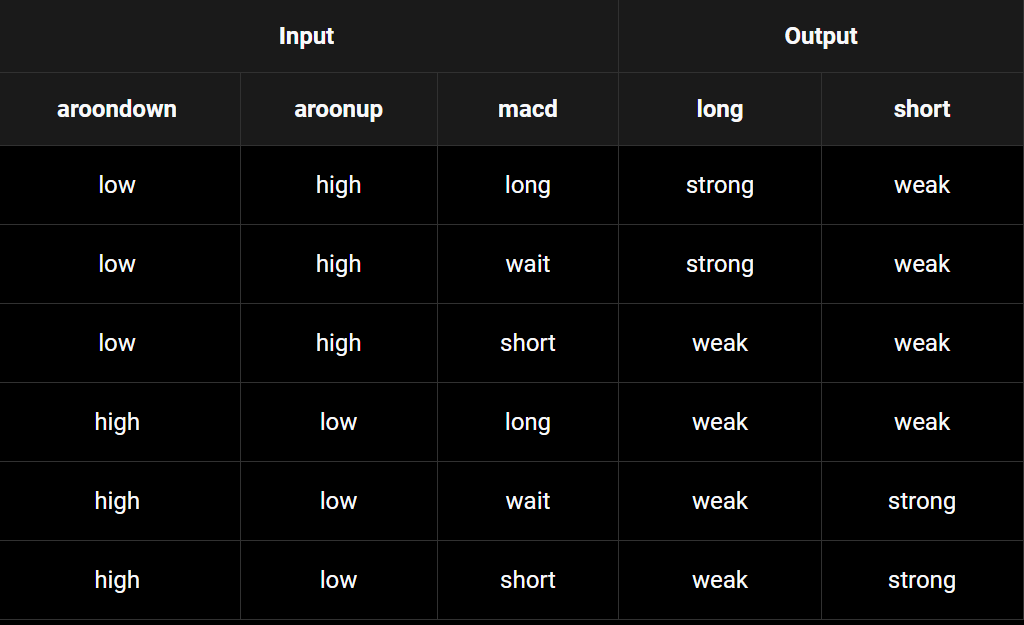
\includegraphics[width=\textwidth]{images/aroon-macd-rules.png}
    \caption{Fuzzy Rules ของตัวชี้วัด AROON-MACD}
    \label{fig:aroon-macd-rules}
\end{figure}
โดยสำหรับตัวชี้วัดนี้จะเป็นตัวชี้วัดแบบ Trend Following ซึ่งคือการที่เราพยายามซื้อขายสินทรัพย์ตามแนวโน้มของตลาด ถ้าตลาดกำลังอยู่ในขาขึ้นก็จะมีการทำการเข้าซื้อแบบ long และถ้าตลาดกำลังอยู่ในขาลงก็จะมีการทำการเข้าซื้อแบบ short โดย MACD จะเป็นตัวที่บอกเราว่าควรเข้าซื้อ ณ เวลาไหน และ AROON จะเป็นตัวบอกเราว่าตลาดกำลังอยู่ในขาขึ้นหรือขาลง โดยเราจะเข้าซื้อเมื่อค่าของอินดิเคเตอร์มีค่าเกิน 30

\subsection{ตัวชี้วัด RSI-BB}
\begin{table}[ht]
    \centering
    \begin{tabular}{lllll}
        \hline
           & RSI   & BB     & Long & Short \\ \hline
        If & $<30$ & $<-80$ & $1$  &       \\ \hline
        If & $>70$ & $>80$  &      & $1$   \\ \hline
    \end{tabular}
    \caption{วิธีการเข้าซื้อแบบ Classical ของตัวชี้วัด RSI-BB}
\end{table}

สำหรับตัวชี้วัดตัวนี้จะมีตัวแปรทางภาษาตามรูปที่ \ref{fig:rsi-bb-lin} ในภาคผนวก และมี Fuzzy Rules ดังรูปที่ \ref{fig:rsi-bb-rules}
\begin{figure}[!ht]
    \centering
    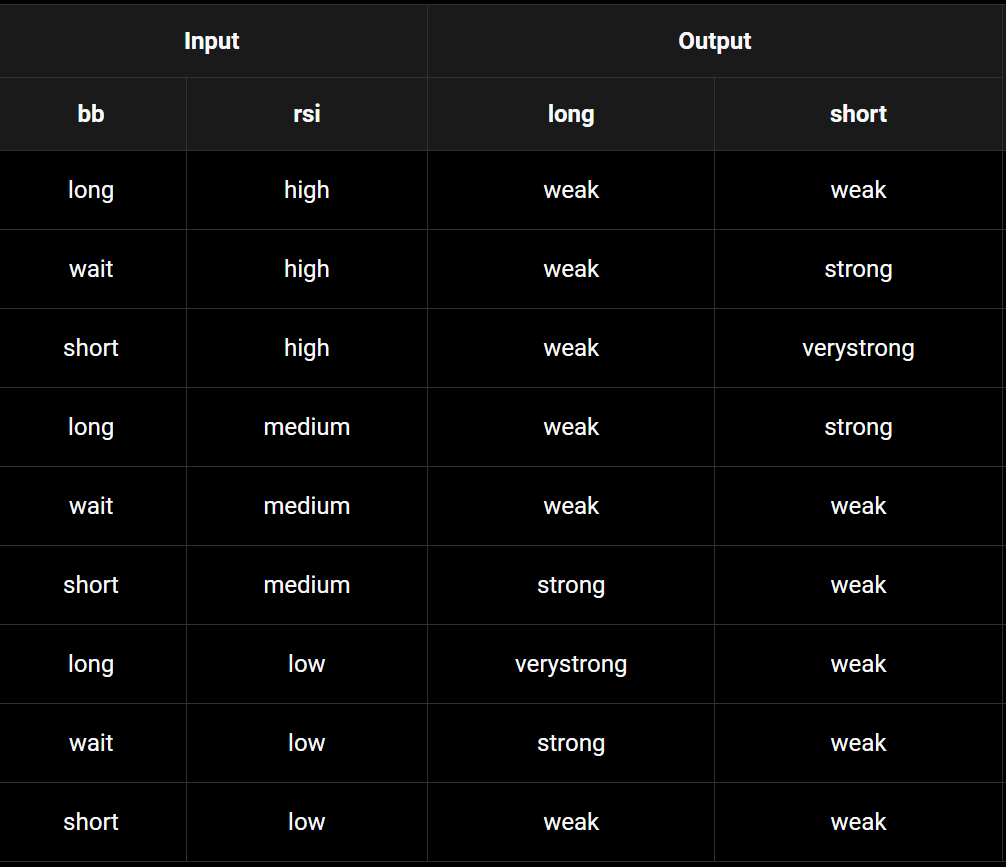
\includegraphics[width=0.8\textwidth]{images/rsi-bb-rules.png}
    \caption{Fuzzy Rules ของตัวชี้วัด RSI-BB}
    \label{fig:rsi-bb-rules}
\end{figure}
โดยสำหรับตัวชี้วัดนี้จะเป็นตัวชี้วัดแบบ Mean Reversion ซึ่งคือการที่เราคาดว่าราคาของสินทรัพย์จะมีแนวโน้มที่จะกลับมาสู่ราคาเฉลี่ย โดย Bollinger Band (BB) จะเป็นตัวบอกว่าราคาของสินทรัพย์นั้นสูงหรือต่ำกว่าค่าเฉลี่ยเกินไปหรือไม่ และ RSI จะเป็นตัวที่บอกเราว่าควรเข้าซื้อ ณ ตอนไหน ถ้าราคาของสินทรัพย์นั้นต่ำกว่าค่าเฉลี่ย และ RSI บอกว่าสินทรัพย์นั้นมีการขายอย่างมาก เราก็จะเข้าซื้อแบบ long และถ้าราคาของสินทรัพย์นั้นสูงกว่าค่าเฉลี่ย และ RSI บอกว่าสินทรัพย์นั้นมีการซื้ออย่างมาก เราก็จะเช้าซื้อแบบ short โดย เราจะเข้าซื้อเมื่อค่าของอินดิเคเตอร์นี้มีค่าเกิน 25

\section{ผลการทดลอง}
\begin{table}[!htb]
    \centering
    \begin{tabular}{crrrrr}
        \hline
        \textbf{Symbol} & \textbf{Classical} & \textbf{Fuzzy} & \textbf{Fuzzy C} & \textbf{Fuzzy PSO} & \textbf{Fuzzy PSO C} \\ \hline
        BTC             & 680.48             & 654.28         & 1035.67          & 1383.01            & \textbf{1450.66}     \\ \hline
        ETH             & 440.45             & 509.39         & 509.16           & 294.08             & \textbf{1264.20}     \\ \hline
        BNB             & 448.98             & 496.05         & 736.79           & 554.83             & \textbf{926.30}      \\ \hline
        TOTAL           & 1569.91            & 1659.72        & 2281.62          & 2231.92            & \textbf{3641.15}     \\ \hline
    \end{tabular}
    \caption{ผลกำไรขาดทุนของการทดสอบตัวชี้วัด AROON-MACD ในตลาด Crypto Currency (หน่วยเป็น USD) ด้วยกรอบเวลา 1 ชั่วโมง (1h)}
    \label{tab:aroon-macd-crypto}
\end{table}

\begin{table}[!htb]
    \centering
    \begin{tabular}{crrrrr}
        \hline
        \textbf{Symbol} & \textbf{Classical} & \textbf{Fuzzy} & \textbf{Fuzzy C} & \textbf{Fuzzy PSO} & \textbf{Fuzzy PSO C} \\ \hline
        AAPL            & \textbf{4.41}      & 0.37           & -0.01            & -18.55             & -23.70               \\ \hline
        IBM             & \textbf{81.12}     & 62.58          & 28.71            & 74.48              & 75.30                \\ \hline
        JPM             & 13.59              & \textbf{20.73} & 20.72            & 7.41               & -10.78               \\ \hline
        MSFT            & \textbf{90.80}     & 64.01          & 64.80            & 59.54              & 6.60                 \\ \hline
        NKE             & \textbf{45.31}     & 23.76          & 23.68            & 23.71              & -27.81               \\ \hline
        TSLA            & \textbf{171.23}    & 59.16          & 56.97            & 6.73               & -3.14                \\ \hline
        TOTAL           & \textbf{406.46}    & 230.62         & 194.87           & 153.30             & 16.47                \\ \hline
    \end{tabular}
    \caption{ผลกำไรขาดทุนของการทดสอบตัวชี้วัด AROON-MACD ในตลาดหุ้น NASDAQ (หน่วยเป็น USD) ด้วยกรอบเวลา 1 ชั่วโมง (1h)}
    \label{tab:aroon-macd-stocks}
\end{table}
\FloatBarrier
\pagebreak

\begin{table}[!htb]
    \centering
    \begin{tabular}{crrrrr}
        \hline
        \textbf{Symbol} & \textbf{Classical} & \textbf{Fuzzy} & \textbf{Fuzzy C} & \textbf{Fuzzy PSO} & \textbf{Fuzzy PSO C} \\ \hline
        BTC             & -110.64            & -105.57        & -96.40           & 1381.81            & \textbf{1466.41}     \\ \hline
        ETH             & -84.48             & -24.46         & -49.72           & \textbf{1261.53}   & -49.72               \\ \hline
        BNB             & -109.26            & 28.17          & 20.36            & 28.17              & \textbf{1044.98}     \\ \hline
        TOTAL           & -304.38            & -101.87        & -125.76          & \textbf{2671.50}   & 2461.67              \\ \hline
    \end{tabular}
    \caption{ผลกำไรขาดทุนของการทดสอบตัวชี้วัด RSI-BB ในตลาด Crypto Currency (หน่วยเป็น USD) ด้วยกรอบเวลา 1 ชั่วโมง (1h)}
    \label{tab:rsi-bb-crypto}
\end{table}

\begin{table}[!htb]
    \centering
    \begin{tabular}{crrrrr}
        \hline
        \textbf{Symbol} & \textbf{Classical} & \textbf{Fuzzy} & \textbf{Fuzzy C} & \textbf{Fuzzy PSO} & \textbf{Fuzzy PSO C} \\ \hline
        AAPL            & \textbf{17.09}     & -20.55         & -20.55           & -21.33             & -3.53                \\ \hline
        IBM             & -50.07             & 69.16          & 53.64            & \textbf{172.27}    & 17.32                \\ \hline
        JPM             & -57.70             & \textbf{24.27} & 20.96            & -112.47            & -109.25              \\ \hline
        MSFT            & -25.98             & 37.86          & 41.21            & \textbf{89.50}     & -15.32               \\ \hline
        NKE             & -7.20              & -45.88         & -45.88           & -45.88             & -22.72               \\ \hline
        TSLA            & -14.12             & \textbf{2.70}  & \textbf{2.70}    & -64.64             &
        \textbf{2.70}                                                                                                        \\ \hline
        TOTAL           & -137.99            & \textbf{67.56} & 52.08            & 17.45              & -130.80              \\ \hline
    \end{tabular}
    \caption{ผลกำไรขาดทุนของการทดสอบตัวชี้วัด RSI-BB ในตลาดหุ้น NASDAQ (หน่วยเป็น USD) ด้วยกรอบเวลา 1 ชั่วโมง (1h)}
    \label{tab:rsi-bb-stocks}
\end{table}

\begin{figure}[!htb]
    \centering
    \subfigure[1h]{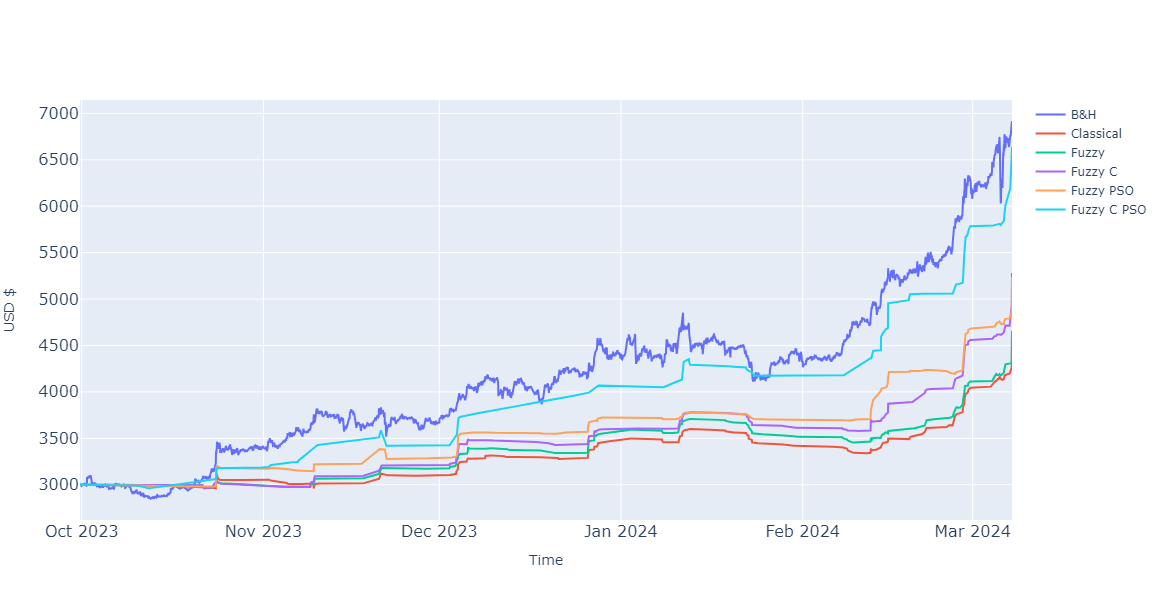
\includegraphics[width=0.95\textwidth]{images/aroon-macd/crypto-result.png}
        \label{fig:aroon-macd-crypto}}
    \subfigure[1d]{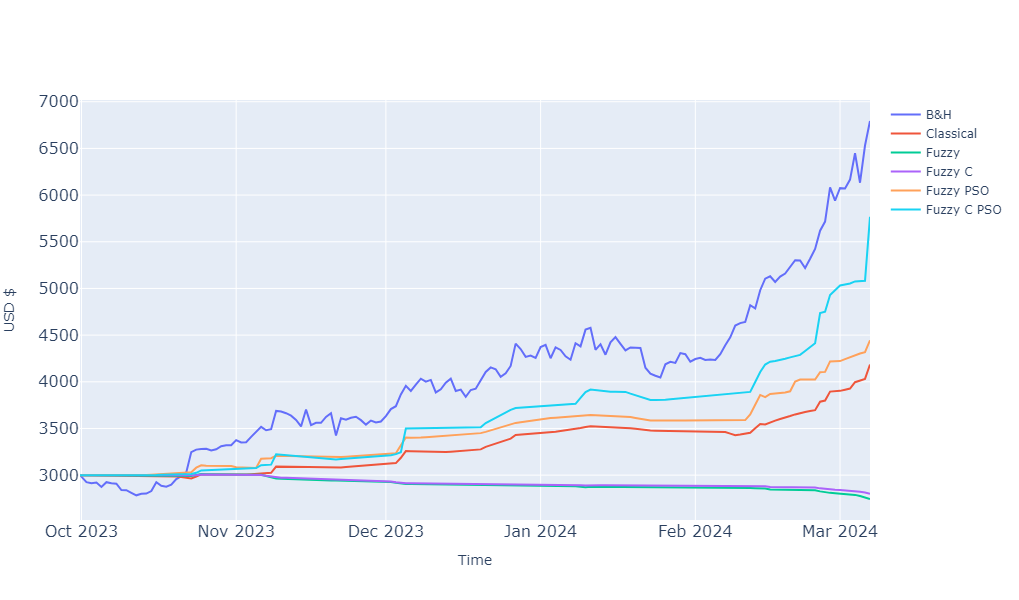
\includegraphics[width=0.95\textwidth]{images/aroon-macd/crypto-result-1d.png}}
    \caption{ความเปลี่ยนของเงินลงทุนของตัวชี้วัด AROON-MACD ในตลาด Crypto Currency ในแต่ละกรอบเวลา}
    \label{fig:aroon-macd-crypto-all}
\end{figure}

\begin{figure}[!htb]
    \centering
    \subfigure[1h]{
        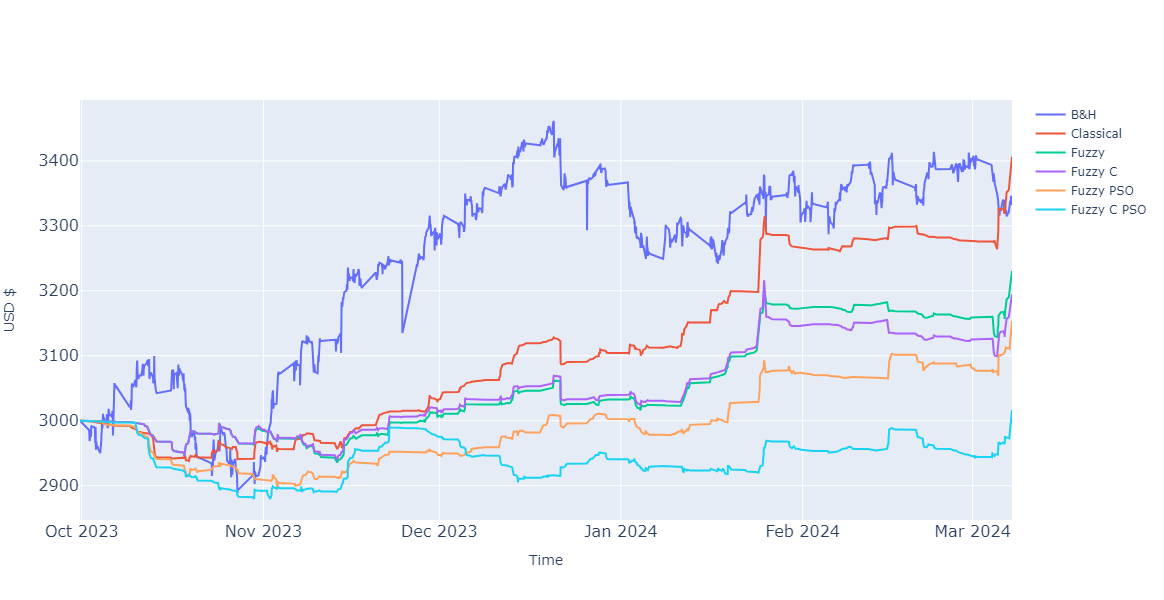
\includegraphics[width=0.95\textwidth]{images/aroon-macd/stock-result.png}
        \label{fig:aroon-macd-stock}
    }
    \subfigure[1d]{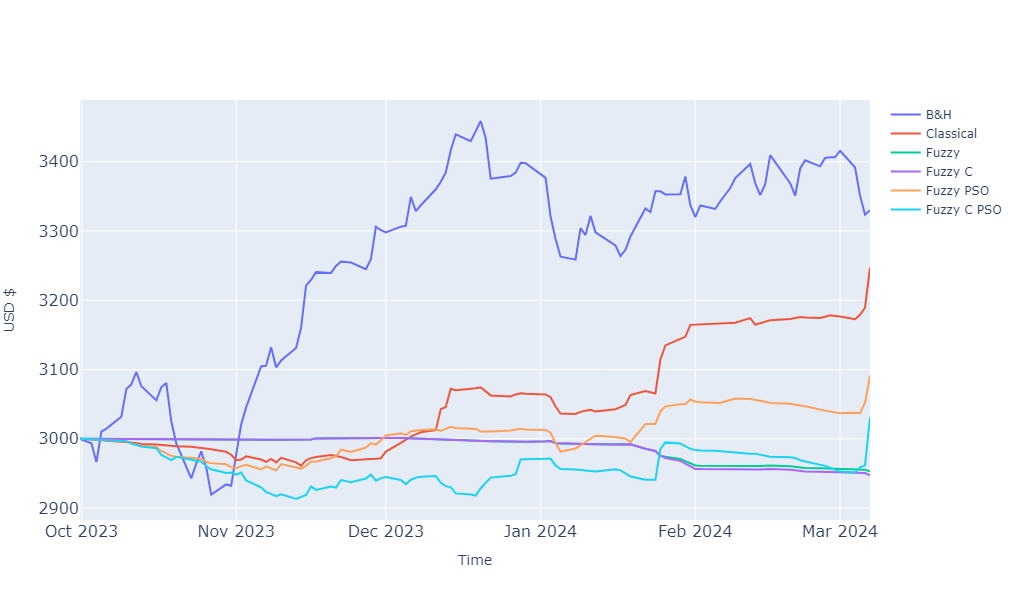
\includegraphics[width=0.95\textwidth]{images/aroon-macd/stock-result-1d.png}}
    \caption{ความเปลี่ยนของเงินลงทุนของตัวชี้วัด AROON-MACD ในตลาดหุ้น NASDAQ ในแต่ละกรอบเวลา}
    \label{fig:aroon-macd-stock-all}
\end{figure}

\begin{figure}[!htb]
    \centering
    \subfigure[1h]{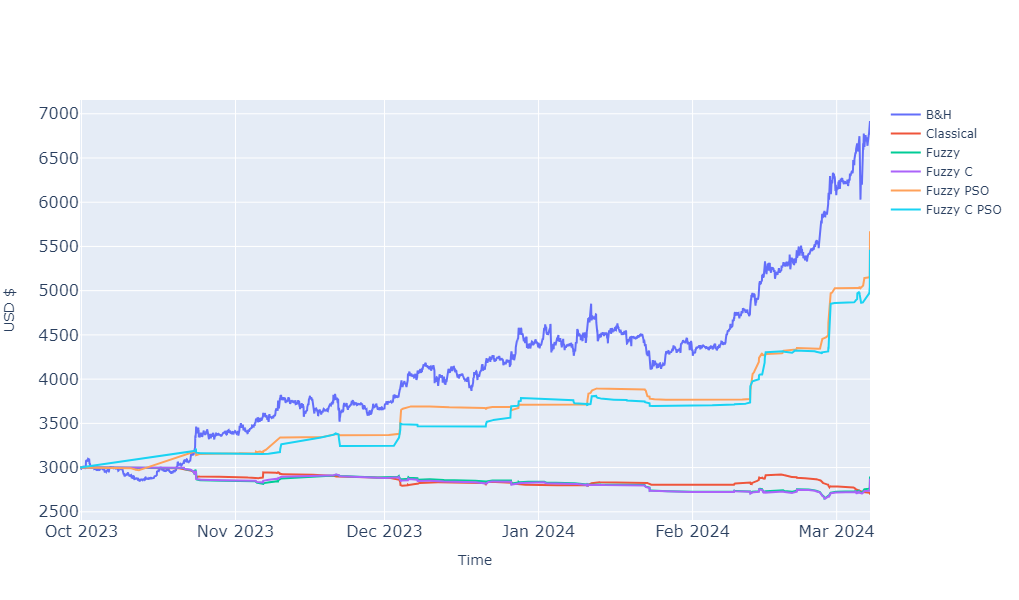
\includegraphics[width=0.95\textwidth]{images/rsi-bb/crypto-result.png}
        \label{fig:rsi-bb-crypto}
    }
    \subfigure[1d]{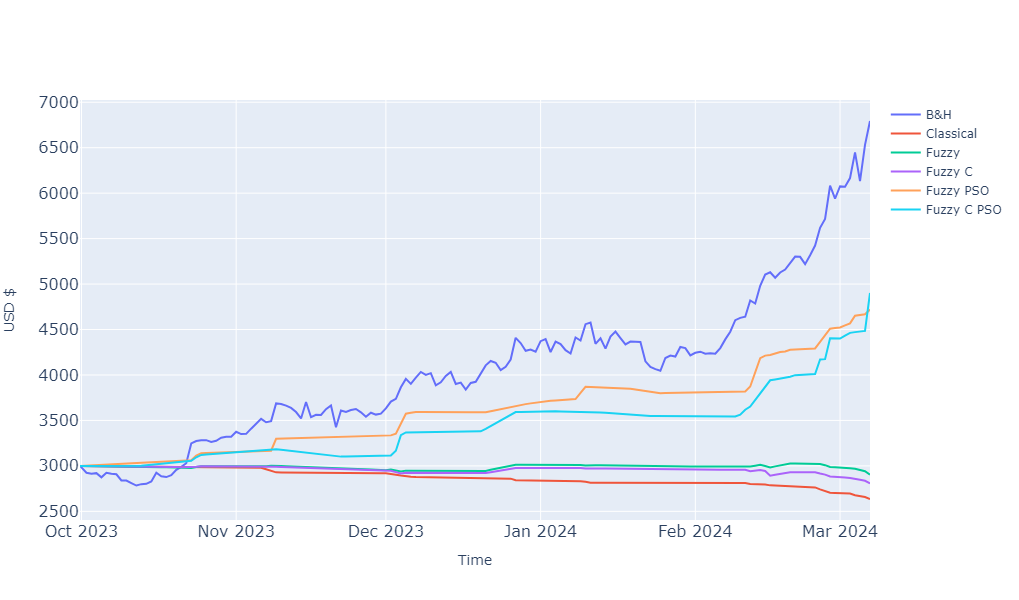
\includegraphics[width=0.95\textwidth]{images/rsi-bb/crypto-result-1d.png}}
    \caption{ความเปลี่ยนของเงินลงทุนของตัวชี้วัด RSI-BB ในตลาด Crypto Currency ในแต่ละกรอบเวลา}
    \label{fig:rsi-bb-crypto-all}
\end{figure}

\begin{figure}[!htb]
    \centering
    \subfigure[1h]{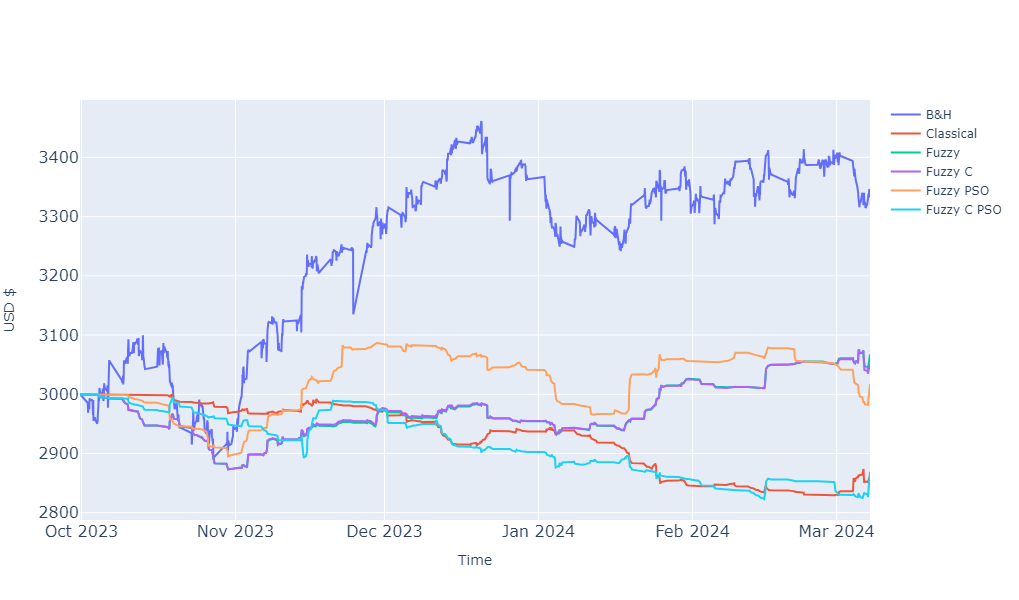
\includegraphics[width=0.95\textwidth]{images/rsi-bb/stock-result.png}
        \label{fig:rsi-bb-stock}
    }
    \subfigure[1d]{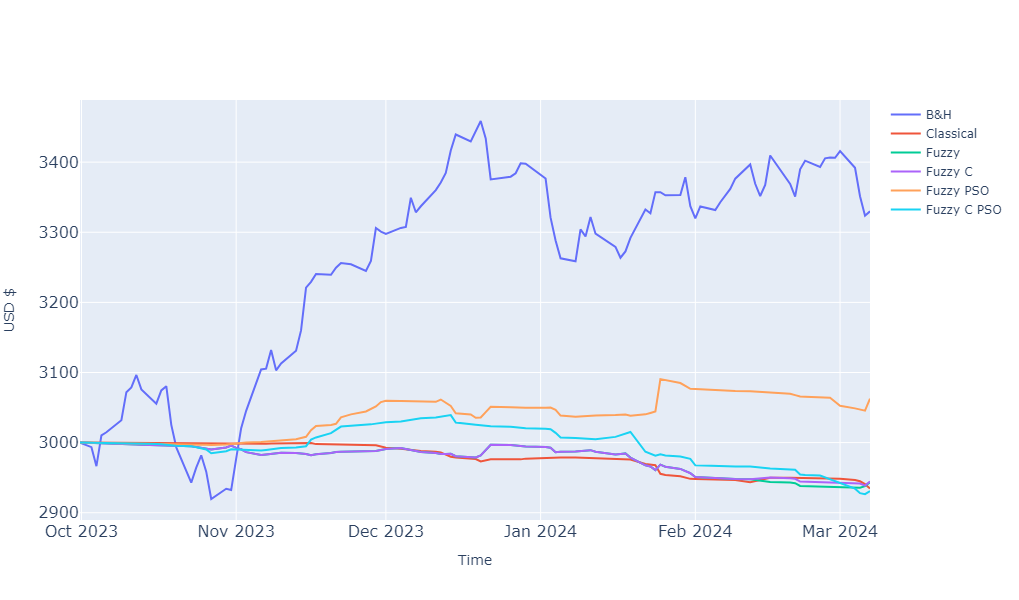
\includegraphics[width=0.95\textwidth]{images/rsi-bb/stock-result-1d.png}}
    \caption{ความเปลี่ยนของเงินลงทุนของตัวชี้วัด RSI-BB ในตลาดหุ้น NASDAQ ในแต่ละกรอบเวลา}
    \label{fig:rsi-bb-stock-all}
\end{figure}

\begin{figure}[!htb]
    \centering
    \subfigure[sideway]{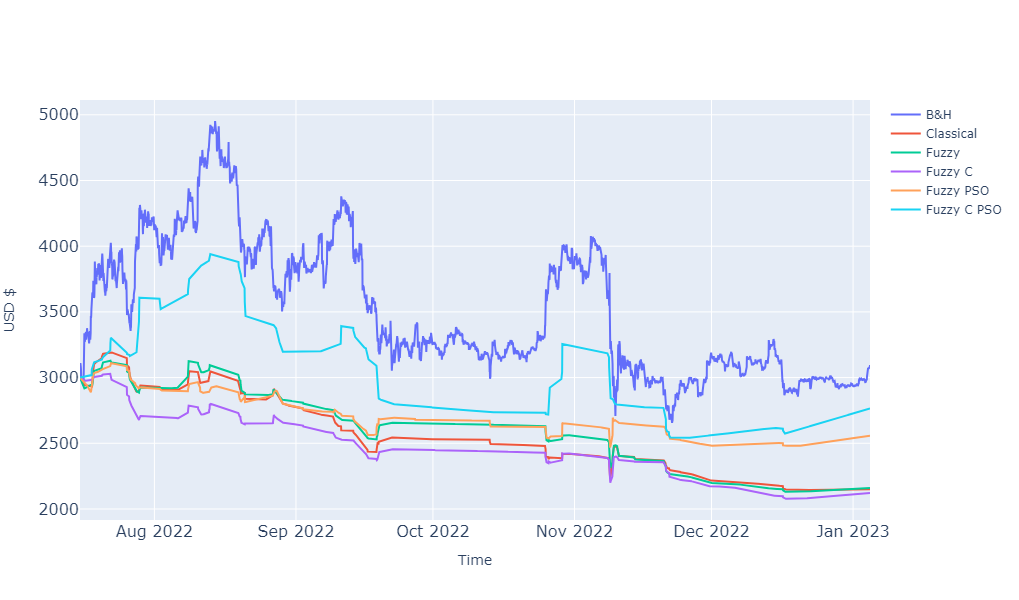
\includegraphics[width=0.95\textwidth]{images/aroon-macd/sideway.png}\label{fig:aroon-macd-side}}
    \subfigure[downtrend]{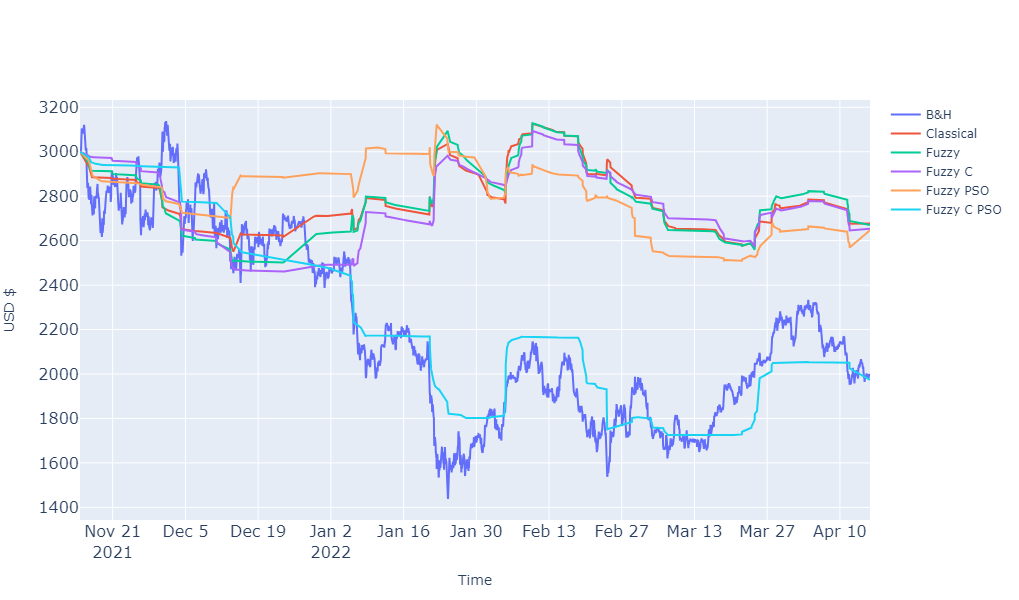
\includegraphics[width=0.95\textwidth]{images/aroon-macd/bear.png}\label{fig:aroon-macd-down}}
    \caption{ความเปลี่ยนของเงินลงทุนของตัวชี้วัด AROON-MACD ในตลาด Crypto Currency (ETH) ในแนวโน้มตลาดแบบทิศทางไม่แน่นอน (sideway) และแบบขาลง (downtrend)}
\end{figure}

\begin{figure}[!htb]
    \centering
    \subfigure[sideway]{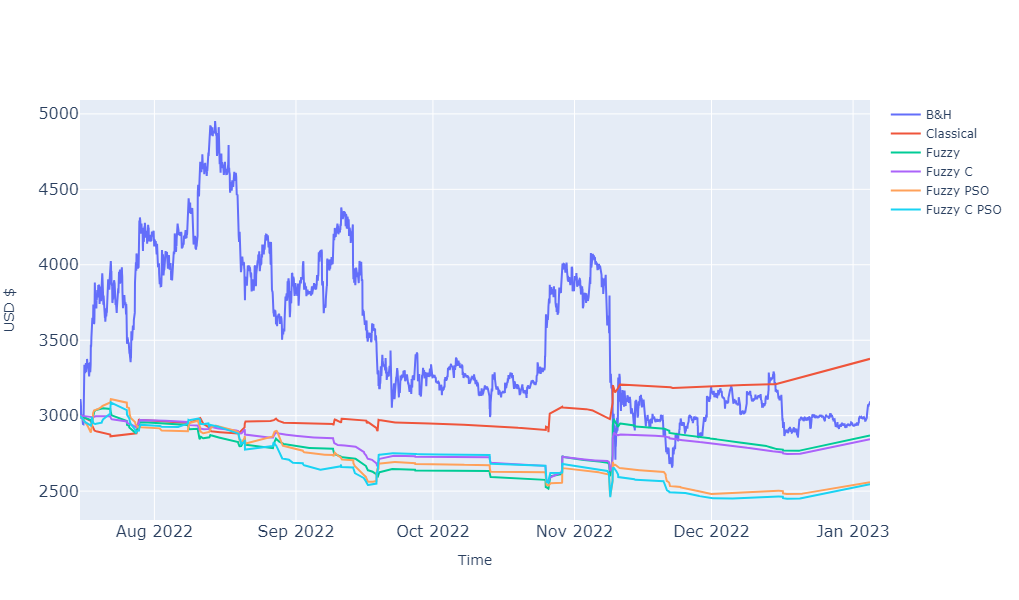
\includegraphics[width=0.95\textwidth]{images/rsi-bb/sideway.png}\label{fig:rsi-bb-side}}
    \subfigure[downtrend]{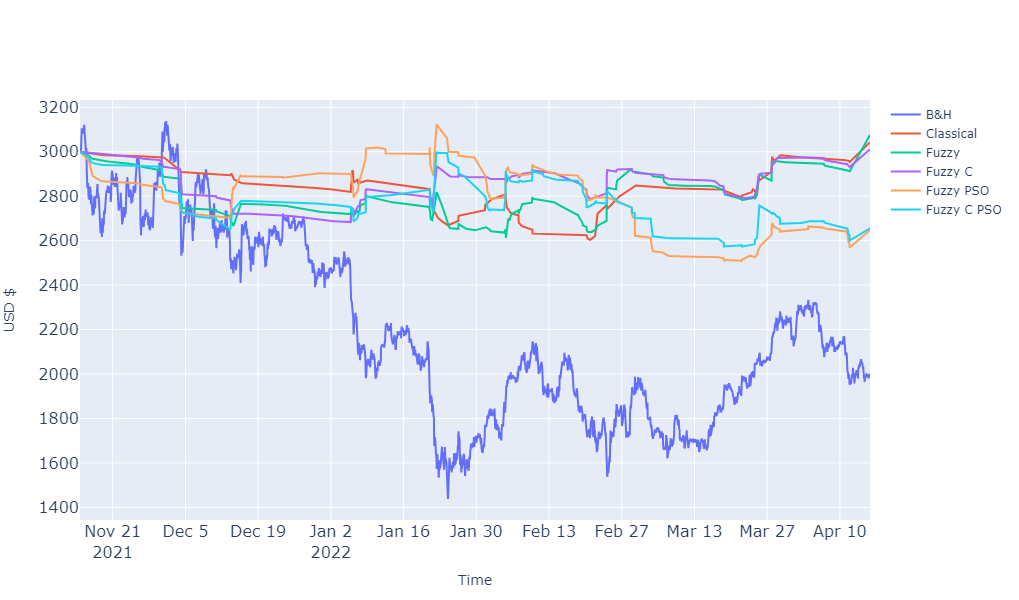
\includegraphics[width=0.95\textwidth]{images/rsi-bb/bear.png} \label{fig:rsi-bb-down}}
    \caption{ความเปลี่ยนของเงินลงทุนของตัวชี้วัด RSI-BB ในตลาด Crypto Currency (ETH) ในแนวโน้มตลาดแบบทิศทางไม่แน่นอน (sideway) และแบบขาลง (downtrend)}
\end{figure}
\FloatBarrier

\section{ผลการวิเคราะห์}
\subsection{ตัวชี้วัด AROON-MACD}
จากตารางที่ \ref{tab:aroon-macd-crypto} และรูปที่ \ref{fig:aroon-macd-crypto} เราจะเห็นว่าการใช้ตัวชี้วัดที่ใช้ Fuzzy Logic นั้นให้ผลลัพธ์ที่ดีกว่าแบบ Classical ในตลาด Crypto Currency ซึ่งจะเห็นว่า Fuzzy PSO C ให้ผลลัพธ์ที่ดีที่สุด โดยอาจจะมาจากการที่ PSO เรียนรู้ว่า Crypto Currency นี้มีแนวโน้มจะขึ้นตลอดดังตัวอย่างของตัวชี้วัดที่ได้จากรูปที่ \ref{fig:aroon-macd-example} ทำให้มีการเข้าซื้อสินทรัพย์แบบ long position เยอะกว่าแบบ short position และในช่วงที่เราทดสอบก็เป็นขาขึ้นของตลาด Crypto Currency ซึ่งทำให้เราได้ผลลัพธ์ที่ดีกว่าอย่างเห็นได้ชัด แต่ก็จะให้เห็นว่ากำไรรวมของตัวชี้วัดที่ใช้ Fuzzy Logic แบบนั้นก็มีค่ามากกว่าแบบ Classical ถึงจะไม่มากเท่ากับแบบ Fuzzy C PSO แต่ในตารางที่ \ref{tab:aroon-macd-stocks} และรูปที่ \ref{fig:aroon-macd-stock} แสดงให้เราเห็นว่าสำหรับในตลาดหุ้น NASDAQ การใช้ตัวชี้วัดที่ใช้ Classical นั้นให้ผลลัพธ์ที่ดีกว่าแบบ Fuzzy Logic โดยเฉพาะในตัวหุ้น TSLA ซึ่งอาจจะมาจากการที่ตลาดมีความผันผวนน้อยกว่าตลาด Crypto Currency ทำให้ข้อดีของ Fuzzy Logic ในการจัดการกับความไม่แน่นอนของตลาดนั้นไม่ได้ช่วยให้ผลลัพธ์ดีขึ้น

\subsection{ตัวชี้วัด RSI-BB}
จากตารางที่ \ref{tab:rsi-bb-crypto} และรูปที่ \ref{fig:rsi-bb-crypto} รวมถึงตารางที่ \ref{tab:rsi-bb-stocks} และ \ref{fig:rsi-bb-stock} จะเห็นว่าการใช้ตัวชี้วัดที่ใช้ Fuzzy Logic นั้นให้ผลลัพธ์ที่กว่าตัวชี้วัดแบบ Classical ทั้งในตลาด Crypto Currency และตลาดหุ้น NASDAQ โดยในตลาด Crypto Currency ตัว Fuzzy PSO จะทำงานได้ดีที่สุดซึ่งเหตุผลก็คล้ายๆ กับที่กล่าวในหัวข้อ AROON-MACD ด้านบนก็คือ PSO นั้นเรียนรู้ว่าตลาด Crypto Currency มีแนวโน้มที่จะขึ้นตลอด ทำให้มีการเข้าซื้อสินทรัพย์แบบ long มากกว่าแบบ short ทำให้ได้กำไรที่ดีกว่ามาก แต่ในตลาดหุ้น NASDAQ นั้นหุ้นแต่ละตัวไม่ได้มีแนวโน้มที่จะขึ้นเหมือนกันทำให้ PSO ไม่ได้เรียนรู้วิธีแบบตลาด Crypto Currency ทำให้ผลลัพธ์ที่ได้ไม่ได้ดีกว่าการใช้แค่ Fuzzy Logic อย่างเดียว ดังนั้นตัว Fuzzy จึงทำงานได้ดีกว่าในตลาดหุ่้น NASDAQ

\subsection{การใช้กรอบของเวลาที่ต่างกัน (1h กับ 1d)}
จากรูปที่ \ref{fig:aroon-macd-crypto-all}, \ref{fig:aroon-macd-stock-all}, \ref{fig:rsi-bb-crypto-all} และ \ref{fig:rsi-bb-stock-all} เราจะเห็นกว่าการใช้กรอบเวลาที่ต่างกัน ไม่ได้ให้ผลลัพธ์ที่แตกต่างจากกันมาก เราจะสังเกตุได้ว่าผลลัพธ์ที่ได้นั้นมีแนวโน้มไปในทางเดียวกันก็คืออันที่ให้ผลลัพธ์ใน 1h ดีอยู่แล้วก็จะให้ผลลัพธ์ใน 1d ดีเช่นกัน แต่ก็จะมีบางอันที่ให้ผลลัพธ์แย่กว่าเดิมเช่นในรูปที่ \ref{fig:rsi-bb-stock-all} จะสังเกตุเห็นว่า Fuzzy C ใน 1h นั้นให้ผลลัพธ์ที่ดีกว่าใน 1d ซึ่งอาจจะมาจากการที่ความถี่ของการเข้าซื้อสินทรัพย์น้อยกว่าทำให้วิธีจัดการเงินทุนแบบ Liquidation F ส่งผลไม่ดี

\subsection{ผลลัพธ์กับตลาดที่มีทิศทางไม่แน่นอน และตลาดขาลง}
สำหรับในตลาดขาลง (downtrend) จะเห็นว่าจากรูปที่ \ref{fig:aroon-macd-down} และ \ref{fig:rsi-bb-down} จะเห็นว่าทั้งแบบ Fuzzy และ Classical นั้นก็ให้ผลลัพธ์ที่ดีกว่าการ Buy \& Hold ไว้ซึ่งก็จะสังเกตุเห็นว่าเส้นกราฟสีเขียว (Fuzzy) นั้นจะเป็นตัวที่ให้ผลลัพธ์ดีที่สุดของทั้ง 2 ตัวชี้วัด แสดงให้เห็นว่าตัวชี้วีแบบ Fuzzy ของเราสามารถจัดการกับตลาดขาลงได้

ในส่วนของตลาดที่มีทิศทางไม่แน่นอน (sideway) จากรูปที่ \ref{fig:aroon-macd-side} นั้นตัวเส้นกราฟสีฟ้า (Fuzzy C PSO) นั้นจะให้ผลลัพธ์ดีที่สุดแต่ก็ไม่สามารถทำกำไรได้มากกว่าการ Buy \& Hold แต่ในรูปที่ \ref{fig:rsi-bb-side} จะเห็นว่าแบบ Classical นั้นให้ผลลัพธ์ที่ดีกว่าแบบ Fuzzy อื่นๆ และการ Buy \& Hold ด้วย แต่ก็จะเห็นว่ารูปแบบการซื้อขายอื่นๆ ก็จะพยายามตามแน้วโน้มของตลาดทำให้ไม่ได้ขาดทุนเยอะมาก แสดงให้เห็นว่าตัวชี้วัดแบบ Fuzzy ของเราสามารถจัดการกับตลาดที่มีทิศทางไม่แน่น่อนได้เช่นกัน